\chapter{Microservices}
\label{chap:Microservices}

\section{Überblick}
\label{sec:überblickMicroservice }
"Modularisierung ist nichts Neues. Schon lange werden große Systeme in kleine Module unterteilt, um Software einfacher zu erstellen, zu verstehen und weiterzuentwickeln. Das Neue: Microservices nutzen als Module einzelne Programme, die als eigene Prozesse laufen. Der Ansatz basiert auf der UNIX-Philosophie. Sie lässt sich auf drei Aspekte reduzieren:"\cite[S. 2]{EWolff2016:Microservices}

\begin{itemize}
    \item Ein Programm soll nur eine Aufgabe erledigen, und das soll es gut machen.
    \item Programme sollen zusammenarbeiten können.
    \item Nutze eine universelle Schnittstelle. In UNIX sind das Textströme.
\end{itemize}
Diese Art der Aufteilung wurde schon lange von großen Unternehmen wie Amazon oder Google genutzt und wurde zu nächst \SOA (SOA) genannt. Jedoch unterscheiden sich Microservices und SOA voneinander. Daher wird SOA im Nächsten Kapitel genauer erläutert und im Kapitel \ref{chap:ergebnisse} die Ergebnisse zusammen gefasst und beide Technologien mit einander verglichen.
\\\\
"Der Begriff Microservices ist nicht fest definiert.[] Als erste Näherung dienen folgende Kriterien:"\cite[S. 2]{EWolff2016:Microservices}

\begin{itemize}
    \item Microservices sind ein Modularisierungskonzept. Sie dienen dazu. ein großes Software-System aufzuteilen - und beeinflussen die Organisation und die Software-Entwicklungsprozesse.
    \item Microservices können unabhängig von Änderungen an anderen Microservices in Produktion gebracht werden.
    \item Microservices können in unterschiedlichen Technologien implementiert sein. Es gibt keine Einschränkung auf eine bestimmte Programmiersprache oder Plattform.
    \item Microservices haben einen eigenen Datenhaushalt: eine eigene Datenbank - oder ein vollständig getrenntes Schema in einer gemeinsamen Datenbank.
    \item Microservices können eigene Unterstützungsdienste mitbringen, beispielsweise eine Suchmaschine oder eine spezielle Datenbank. Natürlich gibt es eine gemeinsame Basis für alle Microservices - beispielsweise die Ausführung virtueller Maschinen.
    \item Microservices sind eigenständige Prozesse - oder virtuelle Maschinen, um auch die Unterstützungsdienste mitzubringen.
    \item Dementsprechend müssen Microservices über das Netzwerk kommunizieren. Dazu nutzen Microservices Protokolle, die lose Kopplung unterstützen. Das kann beispielsweise REST sein - oder Messaging-Lösungen.
\end{itemize}

\section{Gr"o\ss e eines Microservice}
\label{sec:groesseMicroservice}
"Der Name \frqq Microservices\flqq\ verrät schon, dass es um die Servicegröße geht - offensichtlich sollen die Services klein sein."\cite[S. 31]{EWolff2016:Microservices} Es gibt verschiedene Möglichkeiten die Größe von Programmen zu ermitteln. Eine Variante ist zum Beispiel das Zählen von  Lines of Code (LOC), jedoch hat diese Methode auch Nachteile. Denn die Anzahl der Codezeilen hängen stark von der verwendeten Programmiersprache ab. Einige Programmiersprachen benötigen mehr Zeilen Code, um eine bestimmte Tätigkeit abzubilden, als andere.
\\
Die Größe von Services sollte jedoch nicht von zentraler Bedeutung sein, denn eine untere Grenze gibt es für Services nicht. "Wohl aber eine obere Grenze: Wenn der Microservice so groß ist, dass er von einem Team nicht mehr weiterentwickelt werden kann, ist sie zu groß. Ein Team sollte dabei eine Größe haben, wie sie für agile Prozesse besonders gut funktioniert. Das sind typischerweise drei bis neun Personen."\cite[S. 34]{EWolff2016:Microservices}
\\
Bei der Größe eines Services ist jedoch darauf zu achten, das ein Service nicht zu viele oder zu wenige Funktionen besitzt. Wie bereits beschrieben, sind Microservices modulare, lose gekoppelte Services. Wird ein Service zu klein angesetzt, können daraus Abhängigkeiten zu anderen Services entstehen und damit das gesetzt der losen Kopplung verletzten. Besitzt hingegen ein Service zu viele Funktionen, wird es meistens nicht mehr als Microservice angesehen, da es nicht eine, sondern mehrere Aufgaben übernimmt und diese wahrscheinlich nicht mehr gut erledigen kann.

\section{Orchestration vs Choreographie}
\label{sec:orchestrationvschoreographie}
Möchte man ein Microservice System aufbauen, stellt sich immer wieder die Frage, wie einzelne Services Strukturiert werden und wie diese unter einander kommunizieren sollen. Ein bestimmter Vorgang startet in der Regel bei einem Service. Nun muss man entscheiden ob weitere Services hinzugezogen, beziehungsweise informiert werden müssen. Je nach Anwendungsfall muss man sich zwischen Service Orchestration und Choreographie entscheiden. Dabei ist es fast unmöglich ein ganzes Microservice-System aus nur einem der beiden Varianten zu bauen.

\subsection{Orchestration}
\label{subsec:orchestration}
Bei der Orchestration handelt es sich um eine Komposition von Services. Ein Geschäftsprozess wird zwar mit Hilfe von mehreren Services abgebildet, jedoch ist nur ein Service dafür zuständig den Geschäftsprozess durchzuführen.
\newpage
\begin{figure}[htb]
    \centering 
    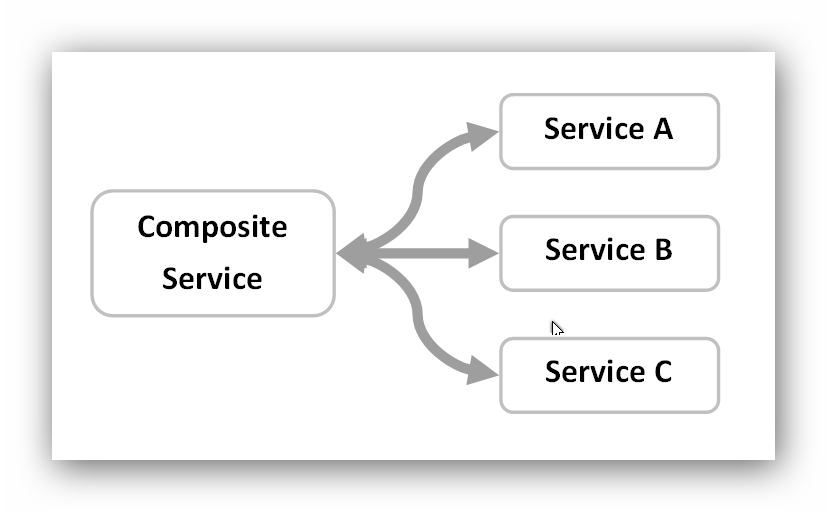
\includegraphics[width=\linewidth]{content/images/ServiceOrchestration}\
    \caption[Orchestration]{Orchestration}
    \label{fig:ServiceOrchestration}  
\end{figure}
\noindent
Wie die Abbildung zeigt besteht \textbf{\underline{keine}} Verbindung zwischen:
\begin{itemize}
    \item A \& B
    \item A \& C
    \item B \& C
\end{itemize}
Nur der "`Composite Service"' nutzt die anderen Microservice um den Geschäftsprozess abzubilden. Diese Art der Kommunikation nennt man Orchestration und wird im Kapitel \secref{chap:soa} noch einmal behandelt.

\subsection{Choreographie}
\label{subsec:choreographie}
Anders als bei der Orchestration können Microservices bei der Choreographie beliebig untereinander kommunizieren. Das ist vor allem dann Sinnvoll, wenn verschiedene Microservice andere Microservice über Änderungen oder andere Aktionen informieren müssen.

\begin{figure}[htb]
    \centering 
    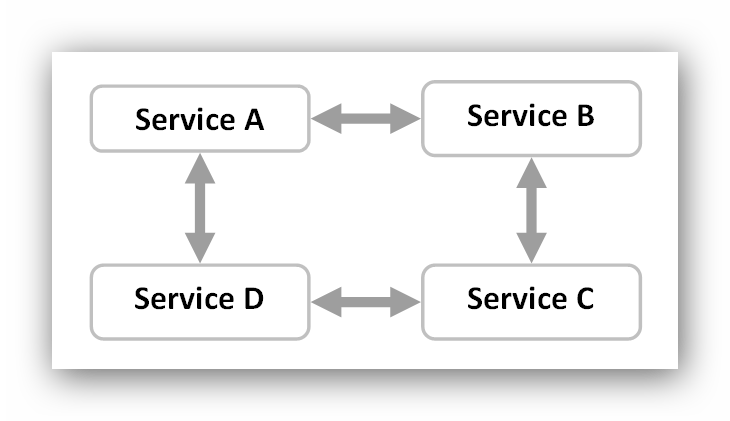
\includegraphics[width=\linewidth]{content/images/ServiceChoreography}\
    \caption[Orchestration]{Orchestration}
    \label{fig:ServiceOrchestration}  
\end{figure}

\section{PUSH- VS PULL-Architektur}
\label{sec:PushPullArchitektur}
Müssen zum Beispiel mehrere Microservices, bei der Durchführung eines Geschäftsprozesses, zusammenarbeiten beziehungsweise über bestimmte Aktionen informiert werden, stellt sich  zunächst die Frage

% [Seite 66 EWolff2016] Technologische Wahlfreiheit
\subsection{Herausforderung}
\label{sec:Herausforderung}
Wie in \cite[S. 25]{EWolff2016:Microservices} beschrieben, besteht ein wesentliches Problem in der Kommunikation zwischen den Services. Der Ausfall eines Services kann im schlechtesten Fall dazu führen, dass alle anderen Microservices nicht mehr funktionieren. Um das zu verhindern, muss klar definiert werden


\section{Continuous-Delivery}
\label{sec:ContinuousDelivery}
"Wer bisher nur Deployment-Monolithen betrieben hat, ist bei Microservices damit konfrontiert, dass es sehr viel mehr deploybare Artefakte gibt, weil jeder Microservice unabhängig in Produktion gebracht wird"\cite[S. 241]{EWolff2016:Microservices}
"Unabhängiges Deployment ist ein zentrales Ziel von Microservices. Außerdem muss das Deployment automatisiert sein, weil ein manuelles Deployment oder auch nur manuelle Nacharbeitung aufgrund der großen Anzahl Microservices nicht umgesetzt werden können"\cite[S. 256]{EWolff2016:Microservices}